\documentclass[a3paper]{article}
\usepackage[utf8]{inputenc}
\usepackage[margin=0.8in]{geometry}

\usepackage{tikz}
\usetikzlibrary{arrows,positioning,shapes.geometric,calc, shapes, shapes.gates.logic.US}

\title{Attack Tools}

\tikzset{
 	headerblock/.style= {draw=none, rectangle, align=center,minimum width=2.5cm,minimum height=0.75cm, fill=gray!30, font=\bf}, 
 	block/.style= {draw, rectangle, align=center,minimum width=2.4cm,minimum height=0.5cm, font=\bfseries}
 }
 
\def \largeX {18cm}
\def \smallY {0.13cm}

\begin{document}
\vspace{10mm}
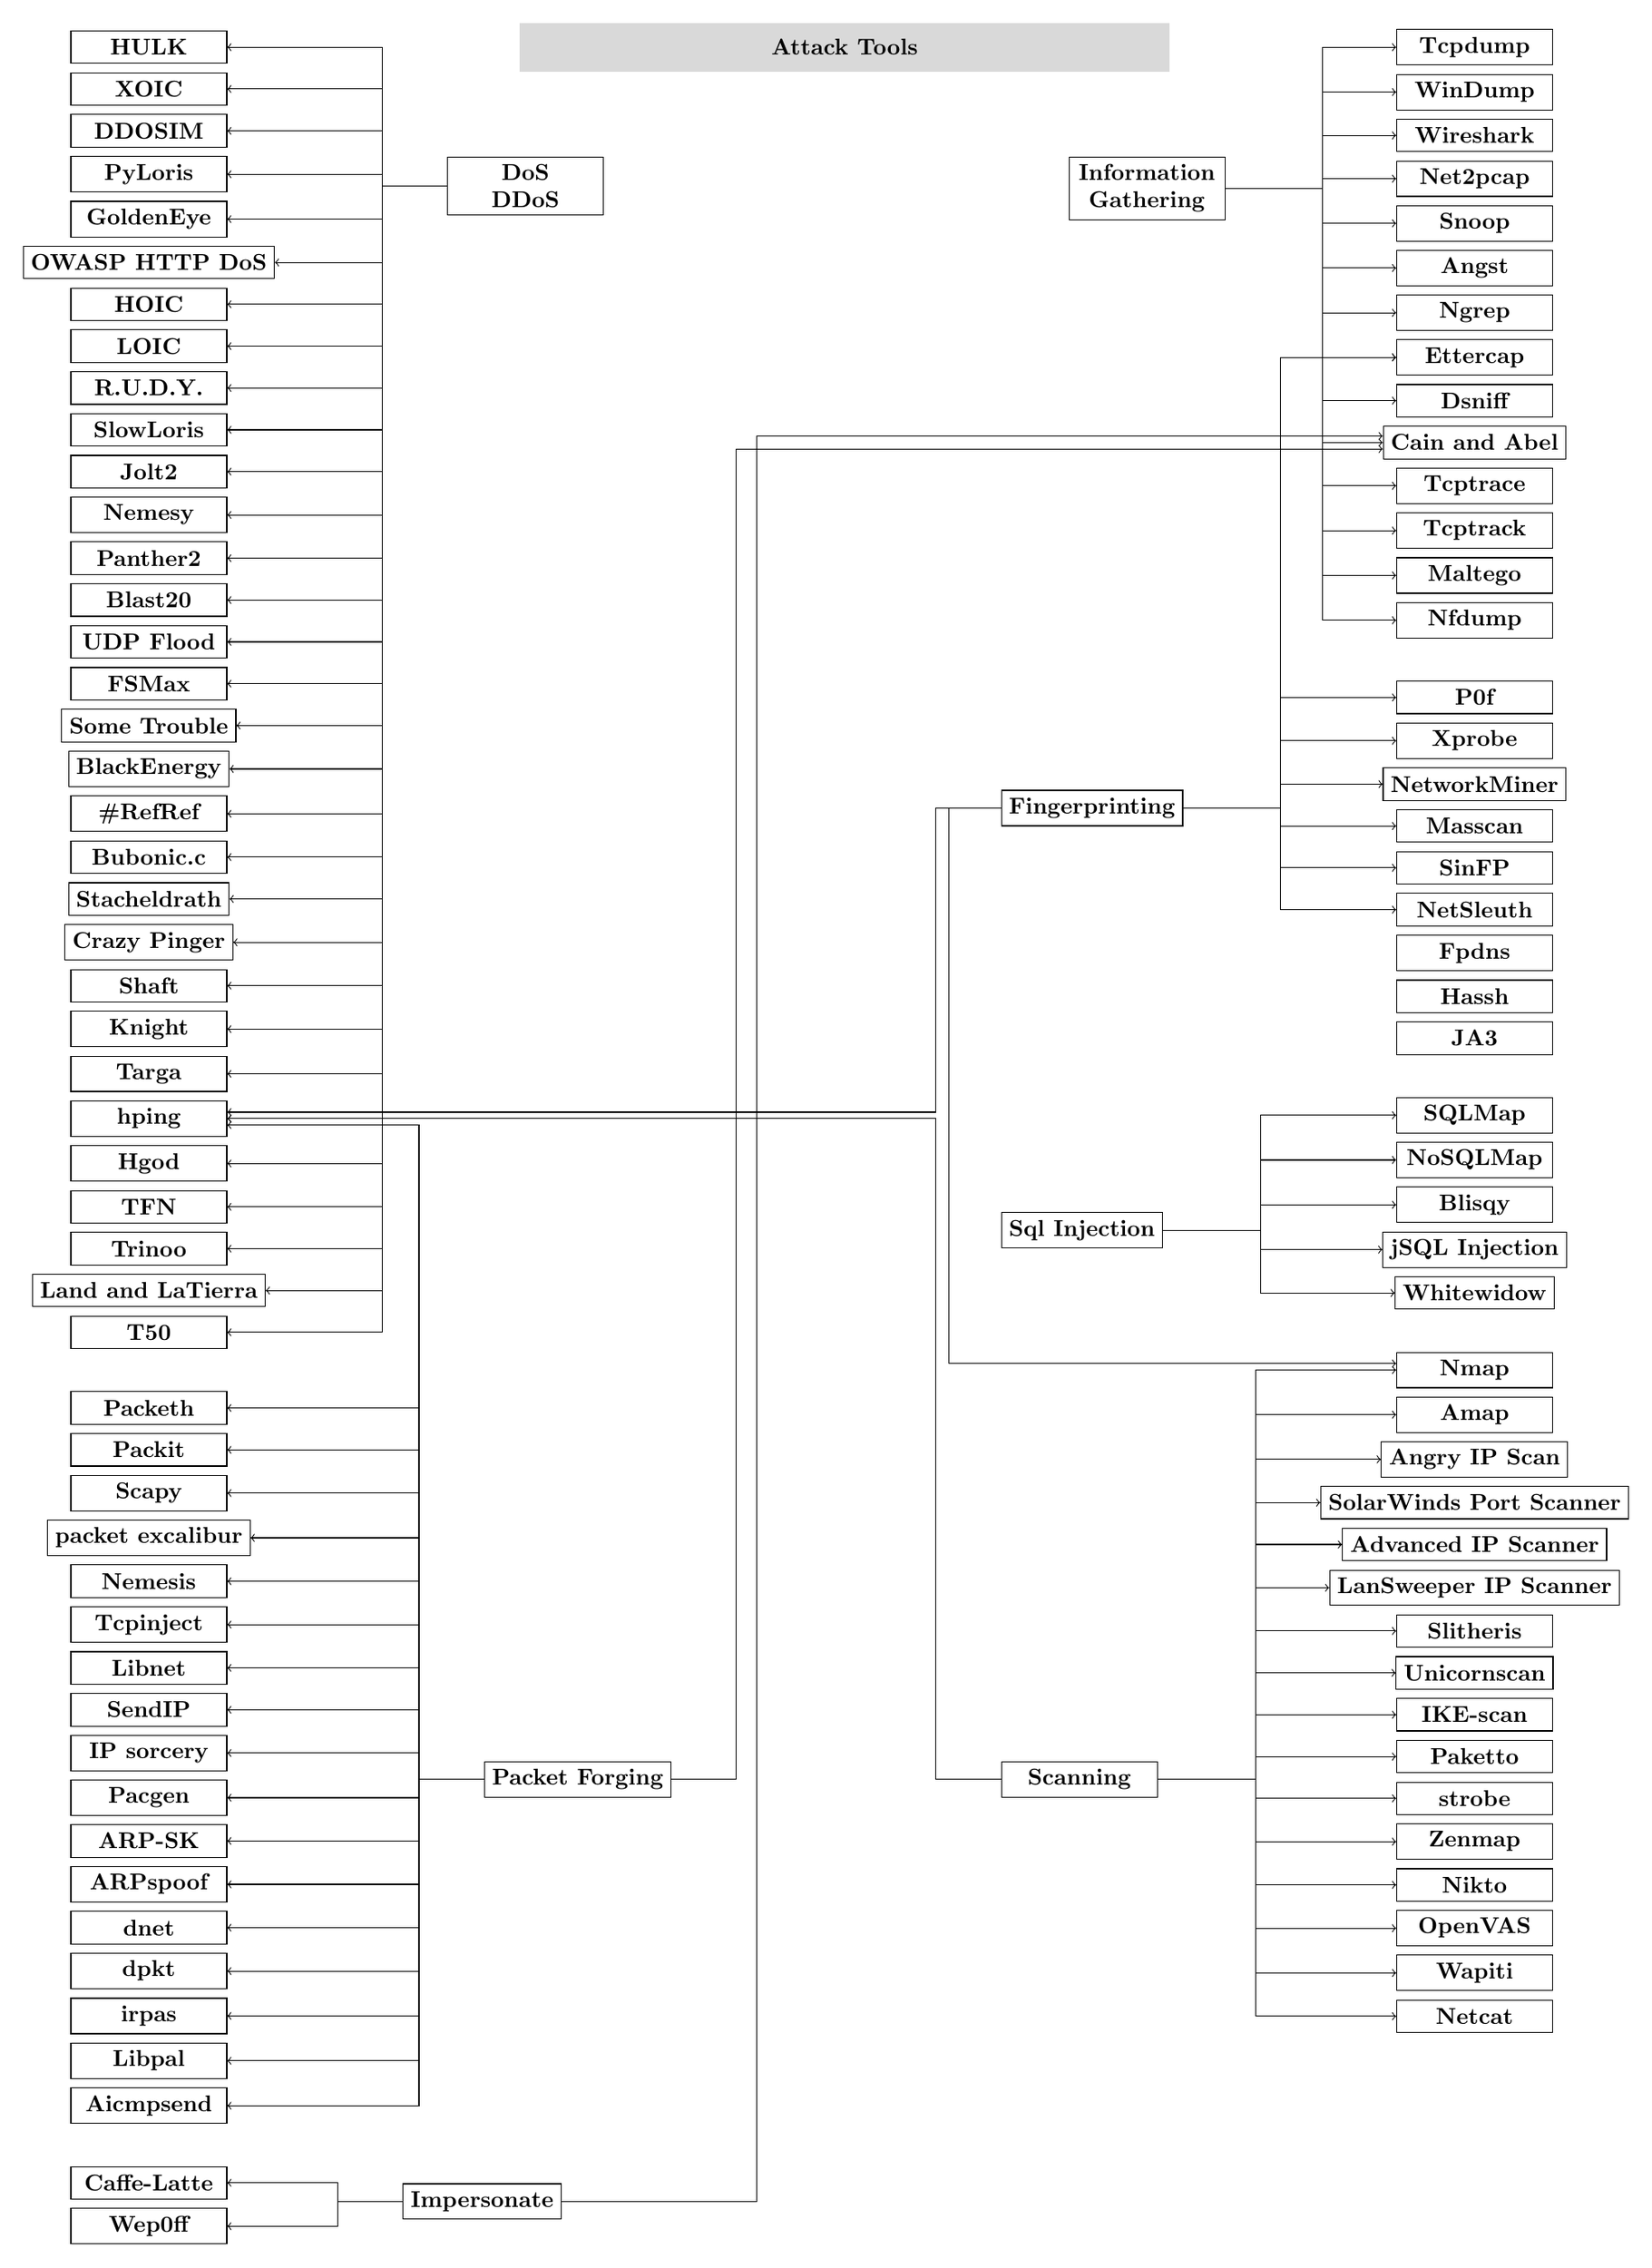
\begin{tikzpicture}
%%%%%%%%%%%%%%%%%%%%% Left Column %%%%%%%%%%%%%%%%%%%%%
    \node [block] (1) {HULK};
    \node [block, below = \smallY of 1] (2) {XOIC};
    \node [block, below = \smallY of 2] (3) {DDOSIM};
    \node [block, below = \smallY of 3] (4) {PyLoris};
    \node [block, below = \smallY of 4] (5) {GoldenEye};
    \node [block, below = \smallY of 5] (6) {OWASP HTTP DoS};
    \node [block, below = \smallY of 6] (7) {HOIC};
    \node [block, below = \smallY of 7] (8) {LOIC};
    \node [block, below = \smallY of 8] (9) {R.U.D.Y.};
    \node [block, below = \smallY of 9] (10) {SlowLoris};
    \node [block, below = \smallY of 10] (11) {Jolt2};
    \node [block, below = \smallY of 11] (12) {Nemesy};
    \node [block, below = \smallY of 12] (13) {Panther2};
    \node [block, below = \smallY of 13] (14) {Blast20};
    \node [block, below = \smallY of 14] (15) {UDP Flood};
    \node [block, below = \smallY of 15] (16) {FSMax};
    \node [block, below = \smallY of 16] (17) {Some Trouble};
    \node [block, below = \smallY of 17] (18) {BlackEnergy};
    \node [block, below = \smallY of 18] (19) {\#RefRef};
    \node [block, below = \smallY of 19] (20) {Bubonic.c};
    \node [block, below = \smallY of 20] (21) {Stacheldrath};
    \node [block, below = \smallY of 21] (22) {Crazy Pinger};
    \node [block, below = \smallY of 22] (23) {Shaft};
    \node [block, below = \smallY of 23] (24) {Knight};
    \node [block, below = \smallY of 24] (25) {Targa};
    \node [block, below = \smallY of 25] (26) {hping};
    \node [block, below = \smallY of 26] (27) {Hgod};
    \node [block, below = \smallY of 27] (28) {TFN};
    \node [block, below = \smallY of 28] (29) {Trinoo};
    \node [block, below = \smallY of 29] (30) {Land and LaTierra};
    \node [block, below = \smallY of 30] (31) {T50};
    

    
    \node [block, below = \smallY*5 of 31] (101) {Packeth};
    \node [block, below = \smallY of 101] (102) {Packit};
    \node [block, below = \smallY of 102] (103) {Scapy};
    \node [block, below = \smallY of 103] (104) {packet excalibur};
    \node [block, below = \smallY of 104] (105) {Nemesis};
    \node [block, below = \smallY of 105] (106) {Tcpinject};
    \node [block, below = \smallY of 106] (107) {Libnet};
    \node [block, below = \smallY of 107] (108) {SendIP};
    \node [block, below = \smallY of 108] (109) {IP sorcery};
    \node [block, below = \smallY of 109] (110) {Pacgen};
    \node [block, below = \smallY of 110] (111) {ARP-SK};
    \node [block, below = \smallY of 111] (112) {ARPspoof};
    \node [block, below = \smallY of 112] (113) {dnet};
    \node [block, below = \smallY of 113] (114) {dpkt};
    \node [block, below = \smallY of 114] (115) {irpas};
    \node [block, below = \smallY of 115] (116) {Libpal};  
    \node [block, below = \smallY of 116] (117) {Aicmpsend};

    \node [block, below = \smallY*5 of 117] (201) {Caffe-Latte};
    \node [block, below = \smallY of 201] (202) {Wep0ff};


    

%     \node [block, below = \smallY of a40] (a41) {Hirte};
%     \node [block, below = \smallY of a41] (a42) {EvilTwin};


% %%%%%%%%%%%%%%%%%%%%% Right Column %%%%%%%%%%%%%%%%%%%%%
    \node [block, right=\largeX of 1] (401) {Tcpdump};
    \node [block, below = \smallY of 401]  (402) {WinDump};    
    \node [block, below = \smallY of 402] (403) {Wireshark};
    \node [block, below = \smallY of 403] (404) {Net2pcap};
    \node [block, below = \smallY of 404] (405) {Snoop};
    \node [block, below = \smallY of 405] (406) {Angst};
    \node [block, below = \smallY of 406] (407) {Ngrep};
    \node [block, below = \smallY of 407] (408) {Ettercap};
    \node [block, below = \smallY of 408] (409) {Dsniff};
    \node [block, below = \smallY of 409] (410) {Cain and Abel};
    \node [block, below = \smallY of 410] (411) {Tcptrace};
    \node [block, below = \smallY of 411] (412) {Tcptrack};
    \node [block, below = \smallY of 412] (413) {Maltego};
    \node [block, below = \smallY of 413] (414) {Nfdump};
    
    
    \node [block, below = \smallY*5 of 414] (501) {P0f};
    \node [block, below = \smallY of 501] (502) {Xprobe};
    \node [block, below = \smallY of 502] (503) {NetworkMiner};
    \node [block, below = \smallY of 503] (504) {Masscan};
    \node [block, below = \smallY of 504] (505) {SinFP};
    \node [block, below = \smallY of 505] (506) {NetSleuth};
    
    %DNS, SSH & SSL
    \node [block, below = \smallY of 506] (507) {Fpdns};
    \node [block, below = \smallY of 507] (508) {Hassh};
    \node [block, below = \smallY of 508] (509) {JA3};
    
    %SQL
    \node [block, below = \smallY*5 of 509] (601) {SQLMap};
    \node [block, below = \smallY of 601] (602) {NoSQLMap};
    \node [block, below = \smallY of 602] (603) {Blisqy};
    \node [block, below = \smallY of 603] (604) {jSQL Injection};
    \node [block, below = \smallY of 604] (605) {Whitewidow};
    
      
     %Scannign
    \node [block, below = \smallY*5 of 605] (301) {Nmap};
    \node [block, below = \smallY of 301] (302) {Amap};
    \node [block, below = \smallY of 302] (303) {Angry IP Scan};
    \node [block, below = \smallY of 303] (304) {SolarWinds Port Scanner};
    \node [block, below = \smallY of 304] (305) {Advanced IP Scanner};
    \node [block, below = \smallY of 305] (306) {LanSweeper IP Scanner};
    \node [block, below = \smallY of 306] (307) {Slitheris};
    \node [block, below = \smallY of 307] (308) {Unicornscan};
    \node [block, below = \smallY of 308] (309) {IKE-scan};
    \node [block, below = \smallY of 309] (310) {Paketto};
    \node [block, below = \smallY of 310] (311) {strobe};
    \node [block, below = \smallY of 311] (312) {Zenmap}; 
    \node [block, below = \smallY of 312] (313) {Nikto};
    \node [block, below = \smallY of 313] (314) {OpenVAS};
    \node [block, below = \smallY of 314] (315) {Wapiti};
    \node [block, below = \smallY of 315] (316) {Netcat}; 
    

   
%%%%%%%%%%%%%%%%%%%%% Attacks %%%%%%%%%%%%%%%%%%%%%
    \node [headerblock, right = \largeX/4 of 1, minimum width = 10cm] (attacks) {\textbf{Attack Tools}};
    \node [block, below left = \smallY*10 and \smallY*-10 of attacks] (dos) {DoS\\DDoS};  
    \node [block, below right = \smallY*10 and \smallY*-12 of attacks] (info) {Information\\Gathering};
    \node [block, below right = \smallY*135 and \smallY*-20 of attacks] (sql) {Sql Injection};
    \node [block, block, below left = \smallY*200 and \smallY*-18 of attacks] (forging) {Packet Forging};
    \node [block, block, below right = \smallY*85 and \smallY*-20 of attacks] (fingerprinting) {Fingerprinting};
    \node [block, block, below left = \smallY*250 and \smallY*-5 of attacks] (impersonate) {Impersonate};
    \node [block, block, below right = \smallY*200 and \smallY*-20 of attacks] (scanning) {Scanning};

% %%%%%%%%%%%%%%%%%%%%%%%%%%%%%%%%%%%%%%%%%%%%%%%%%
% %%%%%%%%%%%%%%%%%%%%% Links %%%%%%%%%%%%%%%%%%%%%
% %%%%%%%%%%%%%%%%%%%%%%%%%%%%%%%%%%%%%%%%%%%%%%%%%

%DoS
 \foreach \x in {1,...,31}
        \draw[->] (dos.west) -- ($(dos.west) - (1, 0)$)  |- (\x.east); 
 
% info gathering        
 \foreach \x in {401,...,414}
        \draw[->] (info.east) -- ($(info.east) - (-1.5, 0)$)  |- (\x.west);


% forging        
 \foreach \x in {101,...,117}
        \draw[->] (forging.west) -- ($(forging.west) - (1, 0)$)  |- (\x.east); 
 
% impersonate        
 \foreach \x in {201,...,202}
        \draw[->] (impersonate.west) -- ($(impersonate.west) - (1, 0)$)  |- (\x.east); 
  
% scanning        
 \foreach \x in {301,...,316}
        \draw[->] (scanning.east) -- ($(scanning.east) - (-1.51, 0)$)  |- (\x.west);
 

 
% fingerprinting        
 \foreach \x in {501,...,506}
        \draw[->] (fingerprinting.east) -- ($(fingerprinting.east) - (-1.5, 0)$)  |- (\x.west);
        
% sql        
\foreach \x in {601,...,605}
    \draw[->] (sql.east) -- ($(sql.east) - (-1.5, 0)$)  |- (\x.west);
        
\draw[->] (forging.west) -- ($(forging.west) - (1, 0)$)  |- ($(26.east) - (0,0.1)$); 
\draw[->] (forging.east) -- ($(forging.east) - (-1, 0)$)  |- ($(410.west) - (0,0.1)$); 

\draw[->] (scanning.west) -- ($(scanning.west) - (1, 0)$)  |- (26.east); 

 \draw[->] (impersonate.east) -- ($(impersonate.east) - (-3, 0)$)  |- ($(410.west) + (0,0.1)$); 

 \draw[->] (fingerprinting.west) -- ($(fingerprinting.west) - (1, 0)$)  |- ($(26.east) + (0,0.1)$); 
 \draw[->] (fingerprinting.west) -- ($(fingerprinting.west) - (0.8, 0)$)  |- ($(301.west) + (0,0.1) $); 
 \draw[->] (fingerprinting.east) -- ($(fingerprinting.east) - (-1.5, 0)$)  |- (408.west);


\end{tikzpicture}
\end{document}

